\documentclass[aspectratio=169, 14pt]{beamer}
\usepackage{xeCJK}
\usepackage{graphicx}
\usepackage[ruled, lined, linesnumbered, commentsnumbered]{algorithm2e}
\usepackage{pgfplots}
\pgfplotsset{compat=1.9}
\usepackage{tikz}
\usetikzlibrary{matrix,shapes,backgrounds,arrows,calc,shadows.blur,fit,positioning}
\usetikzlibrary {arrows.meta}
\usepackage{minted}
\usepackage{fontawesome5}
\usepackage{booktabs}
\usepackage{caption}
\usepackage{hyperref}
\hypersetup{
	colorlinks=true,
	linkcolor=blue,
	filecolor=magenta,
	urlcolor=cyan,
}
\urlstyle{same}
\usetheme{metropolis}
\metroset{block=fill}
\usecolortheme{default}
\definecolor{darkmidnightblue}{rgb}{0.0, 0.2, 0.4}
\definecolor{LightGray}{gray}{0.9}


%------------------------------------------------------------
%This block of code defines the information to appear in the
%Title page
\title[Programming in Python] %optional
{Python程序设计}

\subtitle{Week1: Introduction}

\author[CHEN Zhongpu] % (optional)
{CHEN Zhongpu}

\institute[] % (optional)
{
	School of Computing and Artificial Intelligence \\
	\href{mailto:zpchen@swufe.edu.cn}{zpchen@swufe.edu.cn}
}

\date[] % (optional)
{SWUFE, Fall 2024}

%End of title page configuration block
%------------------------------------------------------------


%------------------------------------------------------------
%The next block of commands puts the table of contents at the 
%beginning of each section and highlights the current section:

% \AtBeginSection[]
% {
%   \begin{frame}
%     \frametitle{Table of Contents}
%     \tableofcontents[currentsection]
%   \end{frame}
% }
%------------------------------------------------------------


\begin{document}

%The next statement creates the title page.
\frame{\titlepage}

% \begin{frame}
% 	\Large $$Data\ Structure + Algorithm = Program$$
% \end{frame}

{
	\usebackgroundtemplate{
		\tikz[overlay, remember picture]
		\node[opacity=0.4, at=(current page.south east), anchor=south east, yshift=2cm,] {
			
\includegraphics[height=0.6\paperheight]{cover}};
	}
	\begin{frame}
		\section{\textcolor{darkmidnightblue}{1. 课程介绍}}
	\end{frame}

}

\begin{frame}
	\frametitle{关于我:陈中普}

	\begin{block}{\faIcon{book} 研究方向}
		时空数据库,大数据分析,向量数据库,大模型应用
	\end{block}

	\begin{block}{\faIcon{building} 办公室}
		格致楼J-310
	\end{block}

	\begin{block}{\faIcon{home} 主页}
		\href{https://zhongpu.info}{https://zhongpu.info}
	\end{block}

\end{frame}
\begin{frame}
	\frametitle{关于课程}
	\begin{block}{Not Only Python}
		本课程面向\underline{没有编程基础}的学生,将围绕着Python语言,讨论程序设计的\alert{术}与\alert{道}。
	\end{block}
	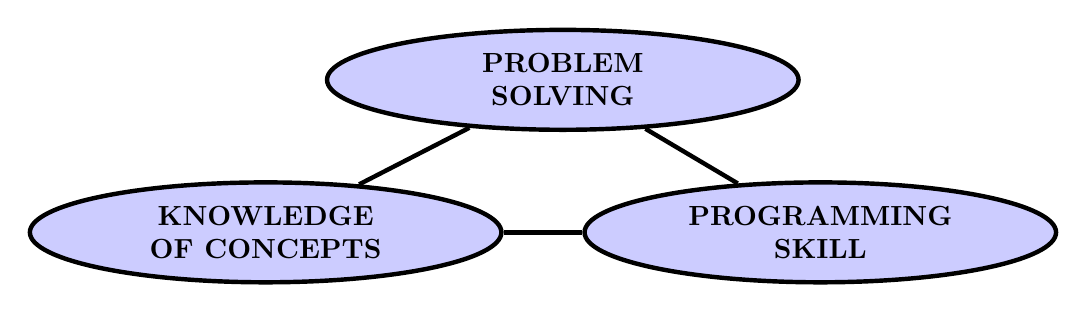
\begin{tikzpicture}
		\tikzstyle{colorn} = [draw, ellipse, ultra thick, fill=blue!20,
		text width=4cm, text centered, font=\bfseries];
		\node[colorn](knowledge) {KNOWLEDGE OF CONCEPTS};
		\node[right=of knowledge, colorn](skill) {PROGRAMMING SKILL};
		\node[above right=of knowledge, colorn, xshift=-1.5cm](solving) {PROBLEM SOLVING};
		\draw[ultra thick] (knowledge) to (skill);
		\draw[ultra thick] (knowledge) to (solving);
		\draw[ultra thick] (skill) to (solving);
	\end{tikzpicture}
\end{frame}

\begin{frame}
	\frametitle{关于Python}
	\begin{block}{Python官网}
		Python is a programming language that lets you work quickly and integrate systems more effectively.
	\end{block}

	\begin{figure}
		\center
		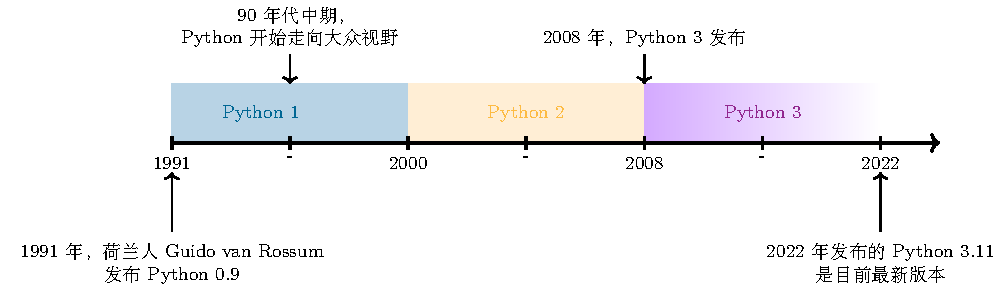
\includegraphics[height=.45\paperheight]{week1/Timeline.pdf}
	\end{figure}
\end{frame}

\begin{frame}
	\begin{exampleblock}{ Pros }
		Python被广泛应用于\alert{科学计算}、\alert{Web开发}、\alert{系统运维}、\alert{人工智能}等领域,是目前最流行的编程语言之一。
	\end{exampleblock}

	\begin{columns}
		\column{0.49\textwidth}
		\begin{tikzpicture}[scale=.75]
			\begin{axis}[
					xlabel=\href{https://www.tiobe.com/tiobe-index/}{Tiobe} 2023年编程语言排名,
					symbolic y coords={Python, C, C++, Java, C\#},
					major y tick style = transparent,
					xmajorgrids=true,
					bar width=10pt,
					enlarge y limits=.2,
					xbar,
					xmin=0, xmax=18, xtick distance=3
				]
				\addplot
				coordinates {
						(16.36,Python)
						(16.26,C)
						(12.91,C++)
						(12.21,Java)
						(5.73,C\#)};
			\end{axis}
		\end{tikzpicture}
		\column{0.49\textwidth}
		\begin{tikzpicture}[scale=.75]
			\begin{axis}[
					xlabel=\href{https://survey.stackoverflow.co/2023/}{StackOverFlow} 2023年语言排名,
					symbolic y coords={JavaScript, HTML\slash{CSS}, Python, SQL, TypeScript},
					major y tick style = transparent,
					xmajorgrids=true,
					bar width=10pt,
					enlarge y limits=.2,
					xbar,
					xmin=30, xmax=70, xtick distance=10
				]
				\addplot [fill=red] coordinates {
						(63.61,JavaScript)
						(52.97,HTML\slash{CSS})
						(49.28,Python)
						(48.66,SQL)
						(38.87,TypeScript)};
			\end{axis}
		\end{tikzpicture}
	\end{columns}

\end{frame}

\begin{frame}
	\begin{exampleblock}{Cons}

		但是\alert{trade-off}总是存在的,Python也有很明显的缺点。
	\end{exampleblock}

	\begin{columns}
		\column{.3\textwidth}
		\begin{tabular}{l c}
			\hline
			\textbf{Language} & \textbf{Time} \\
			\hline
			C                 & 1.00          \\
			Rust              & 1.04          \\
			C++               & 1.56          \\
			Ada               & 1.85          \\
			Java              & 1.89          \\
			Go                & 2.83          \\
			Python            & 71.90         \\
			Lua               & 82.91         \\
			\hline
		\end{tabular}
		\column{.7\textwidth}
		论文\href{https://greenlab.di.uminho.pt/wp-content/uploads/2017/09/paperSLE.pdf}{Energy Efficiency across Programming Languages}表明,在运行时间方面,Python在主流编程语言排名\alert{倒数第二}。
	\end{columns}
\end{frame}

\begin{frame}
	\frametitle{预备知识、考核标准}
	\begin{columns}
		\column{.44\textwidth}
		原则上几乎不需要预备知识,掌握\alert{阅读文档}(尤其是英文文档)和\alert{安装软件}的能力即可。
		\url{https://docs.python.org/3/index.html}
		\column{.56\textwidth}
		\includegraphics[width=\textwidth]{evaluate.pdf}
		\begin{tikzpicture}
			\node[fill=red!80, text=white, blur shadow={shadow xshift=-0.5ex},
				text width=14em,anchor=south west,rounded corners, ]
			{严禁抄袭!多练习!
			};
		\end{tikzpicture}
	\end{columns}
\end{frame}

\begin{frame}
	\frametitle{课程资源}
	参考资料:
	\begin{itemize}
		\item Eric Matthes. \alert{Python Crash Course}. Third Edition. 2022.
		\item \href{https://github.com/ChenZhongPu/python-swufe}{课程代码及课件}
	\end{itemize}

	\begin{figure}
		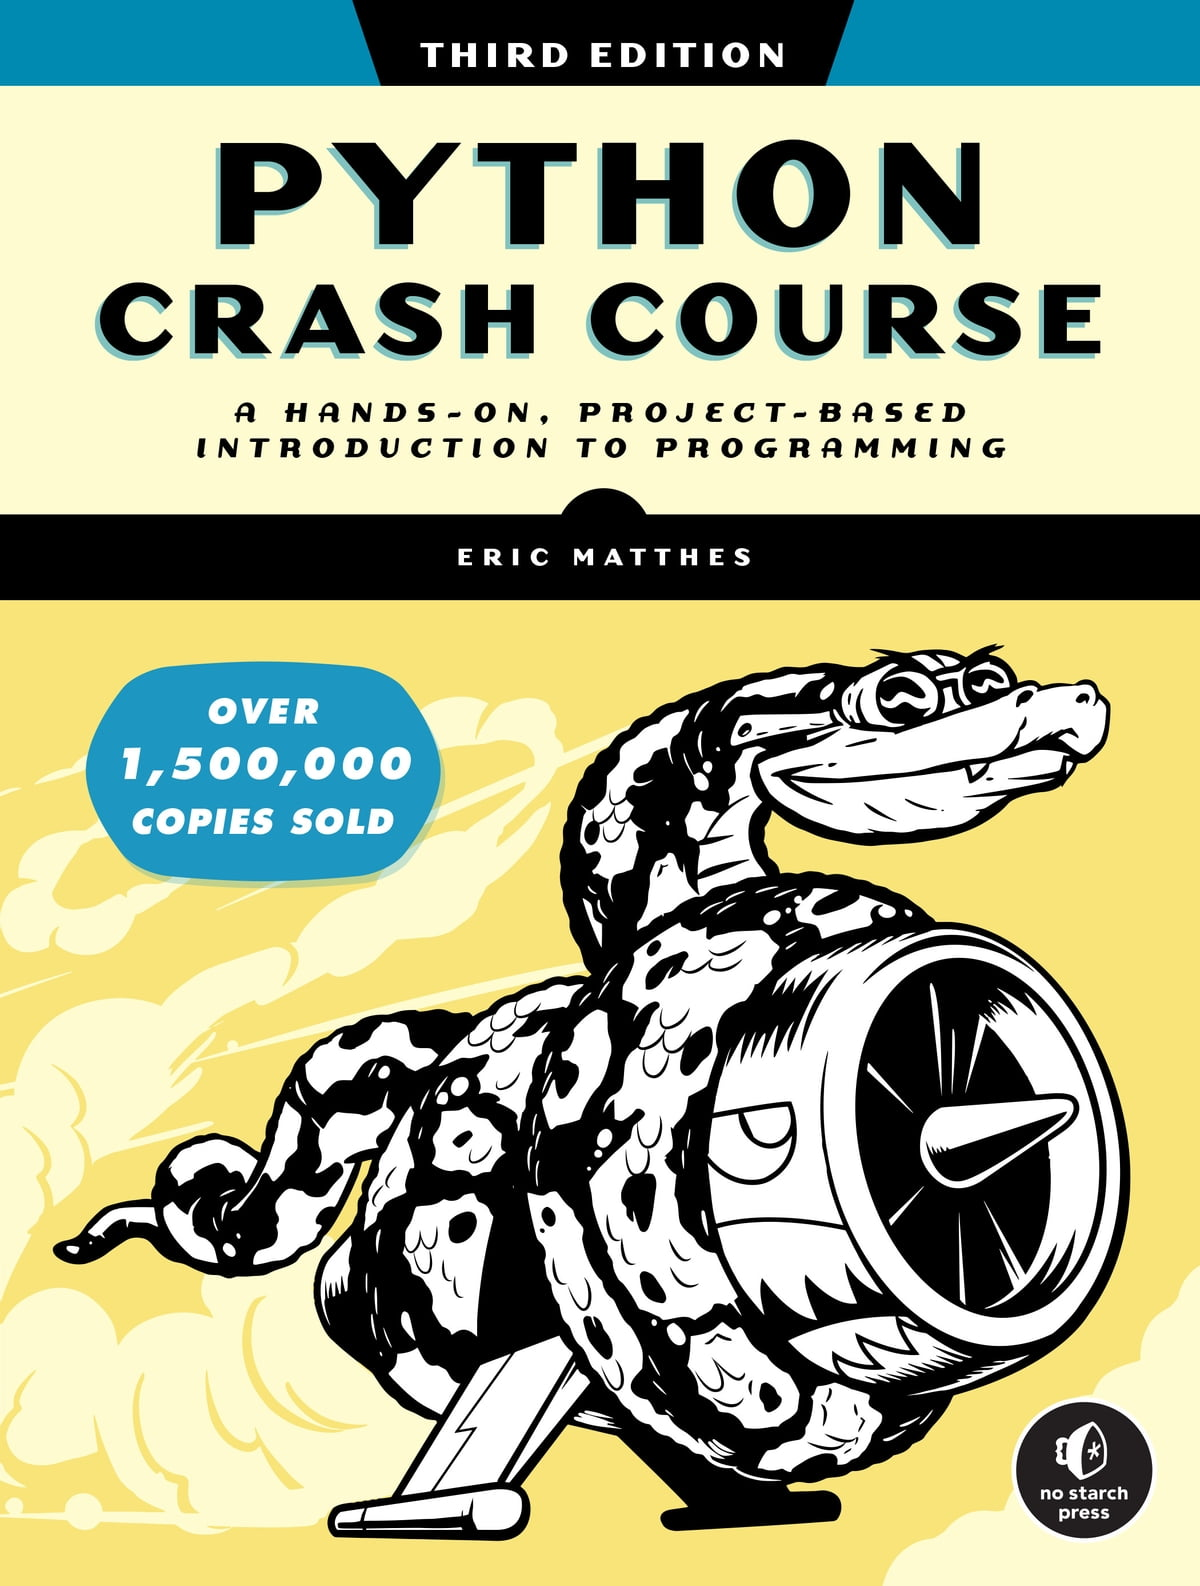
\includegraphics[height=.35\paperheight]{week1/python-crash-course-3rd-edition.jpg}
	\end{figure}

\end{frame}

\begin{frame}{搜索工具}

	\begin{itemize}
		\item StackOverFlow、Google
		\item ChatGPT, Claude
	\end{itemize}

	\begin{quote}
		获取知识的能力比知识本身更有价值。
	\end{quote}

\end{frame}
\begin{frame}
	\frametitle{编程工具}
	本课程推荐使用\alert{Python 3.10+}。

	IDE或编辑器(要求掌握):
	\begin{itemize}
		\item PyCharm (适合专业、大型项目)
		\item VSCode (适合轻量级、小型项目)
		\item Jupyter(适合演示、学习)
	\end{itemize}

	代码AI助手(不要求掌握):
	\begin{itemize}
		\item \url{https://codeium.com}
		\item GitHub CoPilot
	\end{itemize}
\end{frame}

{
\usebackgroundtemplate{
	\tikz[overlay, remember picture]
	\node[opacity=0.4, at=(current page.south east), anchor=south east, yshift=2cm,] {
		
\includegraphics[height=0.6\paperheight]{cover}};
}
\begin{frame}
	\section{\textcolor{darkmidnightblue}{2. 什么是计算?}}
\end{frame}
}

\begin{frame}
	\frametitle{计算、知识与编程}

	\begin{exampleblock}{思考}
		计算机最重要的两个功能是什么?
	\end{exampleblock}
	\begin{figure}
		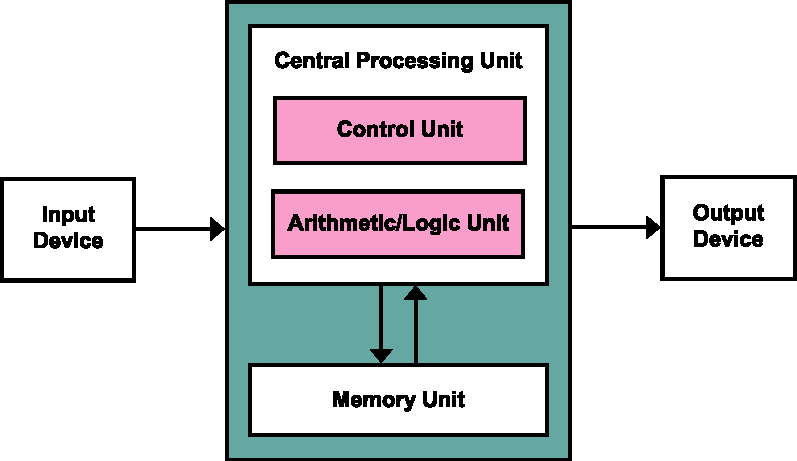
\includegraphics[height=.6\paperheight]{week1/Von_Neumann_Architecture}
	\end{figure}
\end{frame}

\begin{frame}[fragile]
	尽管现代计算机的功能强大(TB级别的存储和GHz级别的CPU),但是计算机只能执行程序员告诉它的任务。换言之,我们需要将\alert{知识注入计算机},而知识的载体就是编程语言。

	\pause
	知识的分类:

	\begin{itemize}
		\item \alert{声明式知识}(declarative knowledge):WHAT
		\item \alert{过程式知识}(imperative knowledge):HOW
	\end{itemize}

	% \begin{tikzpicture}[slot/.style={minimum size=1.2cm,rectangle, fill=blue!30},slot1/.style={minimum size=1.2cm,rectangle, fill=red!30},>=Stealth]
	% 	\matrix [nodes=draw, row sep=0.2cm, column sep=1cm] (one) {
	% 		\node[slot]{算法}; & \node[slot]{控制流}; & \node[slot]{Fixed-program}; & \node[slot]{Stored-program}; \\
	% 	};
	% 	\matrix [nodes=draw, row sep=0.2cm, column sep=1cm, below=of one, yshift=1cm] {
	% 		\node[slot1]{通用图灵机}; &
	% 		\node[slot1]{图灵完备};    \\
	% 	};
	%
	% \end{tikzpicture}

\end{frame}

\begin{frame}
	\frametitle{编程语言与自然语言}
	Each programming language has a set of primitive constructs, a syntax, and a semantics.

	\begin{tabular}{l l p{2in}}
		\toprule
		     & \textbf{自然语言}                     & \textbf{编程语言}                                       \\
		\midrule
		基本构造 & 词汇(cat)                           & 基本数据(\texttt{"cat"}、\texttt{1})和简单操作符({\texttt{+}}) \\
		语法   & I love cats. \alert{I cats love}. & \texttt{1 + 2}, \alert{\texttt{1 2 +}}              \\
		语义   & \alert{I loves cats}.             & \alert{1 + "cat"}                                   \\
		\bottomrule
	\end{tabular}

	% 严格来说,上面的「语义」是\alert{静态语义};任何不符合预期的行为都可以认为是语义错误。
\end{frame}

\begin{frame}[fragile]
	\frametitle{从Hello World开始}
	\begin{minted}[bgcolor=LightGray, baselinestretch=1]{python}
print("Hello World!")
  \end{minted}
	即使本地没有安装Python,也可以通过浏览器在\url{https://replit.com}上运行Python代码。
	\begin{itemize}
		\item \url{https://www.online-ide.com/}
		\item \url{https://www.programiz.com/python-programming/}
		\item \url{https://www.jdoodle.com/}
	\end{itemize}

\end{frame}

\begin{frame}[fragile]

	\begin{minted}[bgcolor=LightGray, baselinestretch=1]{c}
#include <stdio.h>
#include <stdlib.h>
int main(void) {
  printf("Hello World!\n");
  return EXIT_SUCCESS;
}
  \end{minted}

	\begin{minted}[bgcolor=LightGray, baselinestretch=1]{java}
public class Test {
  public static void main(String[] args) {
    System.out.println("Hello World!");
  }
}
  \end{minted}
\end{frame}

\begin{frame}
	\frametitle{几个案例}
	\begin{itemize}
		\item 获取股票价格
		\item 生成二维码
		\item 生成词云
		\item 聊天机器人
	\end{itemize}
\end{frame}

{
\usebackgroundtemplate{
	\tikz[overlay, remember picture]
	\node[opacity=0.4, at=(current page.south east), anchor=south east, yshift=2cm,] {
		
\includegraphics[height=0.6\paperheight]{cover}};
}
\begin{frame}
	\section{\textcolor{darkmidnightblue}{3. Python程序}}
\end{frame}
}

\begin{frame}[fragile]
	\frametitle{基本概念}
	\begin{exampleblock}{程序}
		程序(program)由一系列定义(definition)和命令(command)组成。
	\end{exampleblock}

	\begin{verbatim}
print("Hello, world!")
  \end{verbatim}

	程序所保存的文件被称为\alert{源代码}(source code),在Python中也称\alert{脚本}(script),最后交给Python\alert{解释器}(interpreter)执行,也可以通过Shell执行。
\end{frame}

\begin{frame}
	\frametitle{对象}
	\begin{exampleblock}{对象}
		程序是用来操作数据\alert{对象}(data objects)。对象由\alert{类型}(type)和值(value)构成。不同类型的对象能够执行的操作是不同的。
	\end{exampleblock}

	\pause

	\begin{tikzpicture}
		\node[fill=red!80, text=white, blur shadow={shadow xshift=-0.5ex},
			text width=24em,anchor=south west,rounded corners, ]
		{Python中一切皆对象!换言之,均属于某个类(clsss)。
		};
	\end{tikzpicture}

	对象可大致分为两类:
	\begin{itemize}
		\item \alert{标量}(scalar):不可再分的对象,如整数、浮点数、布尔值,属于\alert{基本数据类型}。
		\item 非标量:可再分的对象,如字符串、列表、字典。
	\end{itemize}


\end{frame}

\begin{frame}
	\frametitle{基本数据类型}
	\begin{tabular}{l l}
		\hline
		\texttt{int}      & 表示整数(integer),比如\texttt{42}                    \\
		\hline
		\texttt{float}    & 表示浮点数(floating-point number),比如\texttt{3.14}   \\
		\hline
		\texttt{bool}     & 表示布尔值(boolean),取值为\texttt{True}和\texttt{False} \\
		\hline
		\texttt{NoneType} & 表示空值(None),只有一个取值\texttt{None}                 \\
		\hline
	\end{tabular}

	\texttt{str}是最简单的\alert{非标量}类型之一,表示字符串(string),比如\texttt{"Hello, world!"}。

\end{frame}

\begin{frame}[fragile]
	\frametitle{类型相关操作}

	\begin{columns}
		\column{.49\textwidth}
		\alert{查看类型}:
		\begin{verbatim}
>>> type(42)
>>> type(3.14)
\end{verbatim}

		\alert{检查类型}:
		\begin{verbatim}
>>> isinstance(42, int)
>>> isinstance(3.14, int)
>>> isinstance(True, int)
\end{verbatim}
		\column{.49\textwidth}
		\alert{转换类型}:
		\begin{verbatim}
>>> int(3.14)
>>> float(42)
>>> float("3.14")
>>> str(3.14)
\end{verbatim}
	\end{columns}

\end{frame}

\begin{frame}
	\frametitle{表达式}
	\begin{exampleblock}{表达式}
		对象和操作符(operator)的组合称为\alert{表达式}(expression),表达式的值也是对象。
	\end{exampleblock}
	算术操作符有:\texttt{+、-、*、/、\%、**};算术表达式的基本格式是:
	$$<\mbox{对象}> <\mbox{操作符}> <\mbox{对象}>$$

	其中,\texttt{/}的结果总是浮点数(整除需要使用\texttt{//});\texttt{\%}的计算不同编程语言不一样;\texttt{**}在其他编程语言中很少见。
\end{frame}

\begin{frame}[fragile]{除法和取余}
	与其他编程语言相比,Python中的整除(又称floor division)和取余操作符有点特殊。
	\begin{verbatim}
>>> 5 / 2
>>> 5 // 2
>>> 5 / -2
>>> 5 // -2
>>> 5 % 2
>>> 5 % -2
>>> -5 % 2
\end{verbatim}
\end{frame}

\begin{frame}[fragile]
	\frametitle{思考}
	下面表达式的结果是什么?
	\begin{verbatim}
>>> 1 + 2 * 3
>>> (1 + 2) * 3
>>> +1
>>> ++++1
>>> -1
>>> ----1
>>> 1 ++++++ 1
\end{verbatim}
\end{frame}

\begin{frame}[fragile]
	\frametitle{变量}
	\begin{exampleblock}{变量}
		值可以通过赋值(assignment)绑定到一个变量(variable);变量是一个\alert{标识符}(identifier),用来引用值。
	\end{exampleblock}

	\begin{columns}
		\column{.4\textwidth}
		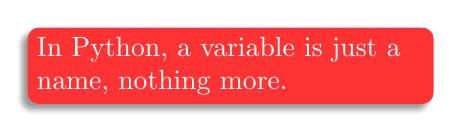
\begin{tikzpicture}
			\node[fill=red!80, text=white, blur shadow={shadow xshift=-0.5ex},
				text width=14em,anchor=south west,rounded corners, ]
			{
				In Python, a variable is just a name, nothing more. };
		\end{tikzpicture}
		\column{.3\textwidth}
		\begin{verbatim}
>>> a = 1
>>> a
>>> a = 2
>>> a = a + 1
>>> b = a
>>> c = d = 42 
  \end{verbatim}
	\end{columns}
\end{frame}

\begin{frame}
	前4个是强制,后2个是建议。
	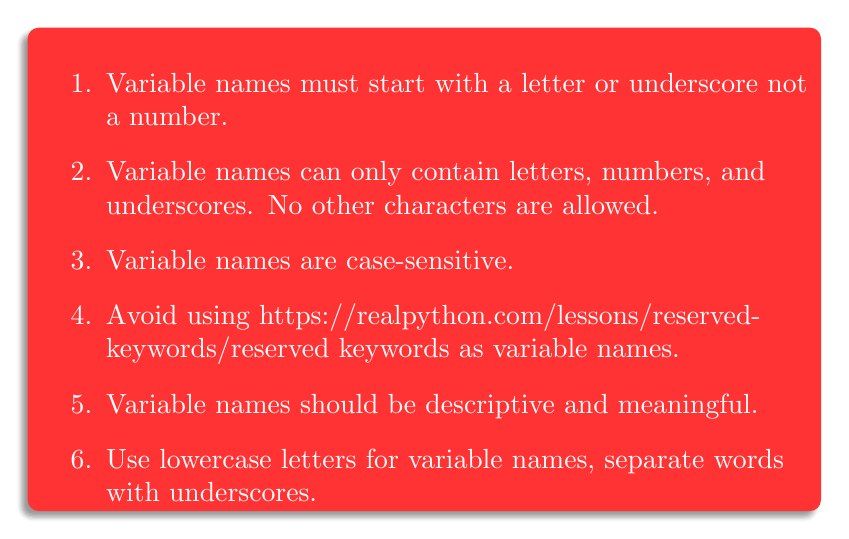
\begin{tikzpicture}
		\node[fill=red!80, text=white, blur shadow={shadow xshift=-0.5ex},
			text width=28em,anchor=south west,rounded corners, ]
		{
			\begin{enumerate}
				\item \textcolor{white}{Variable names must start with a letter or underscore not a number.}
				\item \textcolor{white}{Variable names can only contain letters, numbers, and underscores. No other characters are allowed.}
				\item \textcolor{white}{Variable names are case-sensitive.}
				\item \textcolor{white}{ Avoid using \href{https://realpython.com/lessons/reserved-keywords/}{reserved keywords} as variable names. }
				\item \textcolor{white}{Variable names should be descriptive and meaningful.}
				\item \textcolor{white}{Use lowercase letters for variable names, separate words with underscores.}
			\end{enumerate}
		};
	\end{tikzpicture}
\end{frame}

\begin{frame}[fragile]
	\frametitle{练习与思考}
	考虑下面的Python代码,请定义一个变量来表示圆的面积:

	\begin{minted}[bgcolor=LightGray, baselinestretch=1]{python}
pi = 3.14159
radius = 2.2
# compute the area of an circle
\end{minted}

\end{frame}

\begin{frame}[fragile]
	\frametitle{分支}
	\alert{分支}(branching)是程序中最基本的结构之一,也称为选择结构(selection)。

	\begin{minted}[bgcolor=LightGray, baselinestretch=1]{python}
age = 45
if age > 40:
   salary = 20000
else:
   salary = 18000
print(salary)
\end{minted}

	在上面程序的基础上,进一步掌握比较和逻辑操作符号。
\end{frame}

\begin{frame}
	\frametitle{Tab还是Space}

	通过上面程序,可以看到\alert{缩进}(indentation)在Python中的重要性。

	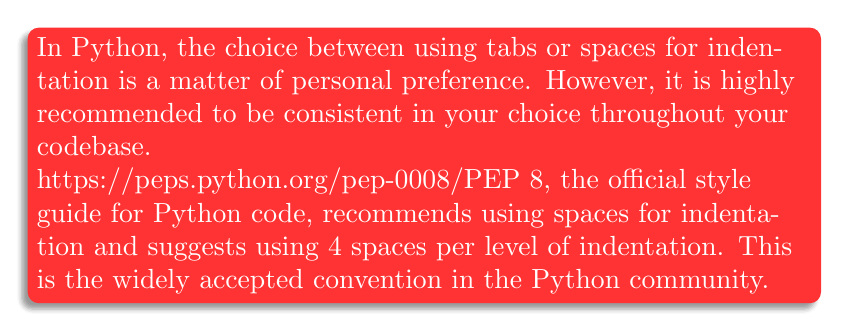
\begin{tikzpicture}
		\node[fill=red!80, text=white, blur shadow={shadow xshift=-0.5ex},
			text width=28em,anchor=south west,rounded corners, ]
		{
			In Python, the choice between using tabs or spaces for indentation is a matter of personal preference. However, it is highly recommended to be consistent in your choice throughout your codebase.

			\href{https://peps.python.org/pep-0008/}{PEP 8}, the official style guide for Python code, recommends using spaces for indentation and suggests using 4 spaces per level of indentation. This is the widely accepted convention in the Python community.
		};
	\end{tikzpicture}
\end{frame}

\begin{frame}[fragile]{三元操作符}
	请搜索资料,使用Python的三元(ternary)操作符实现下面的代码:

	\begin{minted}[bgcolor=LightGray, baselinestretch=1]{python}
age = 45
if age > 40:
   salary = 20000
else:
   salary = 18000
\end{minted}
\end{frame}

\begin{frame}
	\section{\textcolor{darkmidnightblue}{Conclusion}}
	\begin{enumerate}
		\item 什么是计算
		\item Python的特点
		\item 基本数据类型,表达式,变量,分支
	\end{enumerate}
\end{frame}

\begin{frame}
	\frametitle{本周任务}
	\begin{itemize}
		\item 安装Python 3.10+
		\item 安装Visual Studio Code,并安装Python插件
		\item 通过Python Shell或VSCode练习Python
		\item 在Python Shell中输入\alert{import this},并翻译显示的内容
	\end{itemize}
\end{frame}

\begin{frame}{安装JupyterLab}
	建议创建并启动\href{https://docs.python.org/3/tutorial/venv.html}{虚拟环境}后再安装第三方包。\texttt{python -m venv ThePath}
	\begin{block}{第0步}
		配置国内的PIP镜像,如\href{https://mirrors.tuna.tsinghua.edu.cn/help/pypi/}{清华大学}、\href{https://mirror.sjtu.edu.cn/docs/pypi/web/simple}{上海交通大学}。
	\end{block}
	\begin{block}{第1步:安装}
		命令行输入:pip install jupyterlab
	\end{block}
	\begin{block}{第2步:启动}
		命令行输入:jupyter-lab
	\end{block}
\end{frame}
\end{document}
